\chapter{Electronic attachments} \label{chap:attachments}
Attached to the document is the original ART repository in electronic form the original ART source code, as well as the ART handbook and the ARM scene file reference manual. Furthermore, a pre-compiled executable file for the application \texttt{artist} was added to the root directory of the ART source code.

The following directory tree shows the files of the attachment, that are the most interesting to novel users:

\medspace

\dirtree{%
	.1 /.
	.2 \textbf{ART} (Repository folder).
	.3 [...] .
	.3 \textbf{Gallery} (Folder containing example scene files).
	.3 \texttt{artist} (Pre-compiled execution file).
	.3 [...] .
	.2 \textbf{ARM\_Interface.pdf} (The ARM file reference manual).
	.2 \textbf{ART\_Handbook.pdf} (The ART handbook).
}

\chapter{User guide for software}

In this appendix, a user guide for both compiling and running ART with Embree support is provided. 

\subsection{Installing Embree}
\label{embree}
The first thing one has to consider is the installation of Embree. Embree can be obtained via its \href{https://www.embree.org/}{homepage \emph{https://www.embree.org/}} which provides a link to the dedicated \href{https://github.com/embree/embree}{Github repository}. It can either be build from source or installed from pre-compiled binaries. A detailed description of the installation procedure for Windows (32-bit and 64-bit), Linux (64-bit), and macOS (64-bit) can be found in the \texttt{README.md} file in the repository or in the included user documentation \cite{embree2021Doc}.

\subsection{Using ART}
After a successful installation of Embree, ART is ready to be used. A limitation of ART is the fact, that it does only support macOS and Linux systems. However, by installing a Linux subsystem, making ART work on Windows 10 is possible. The next chapter is dedicated to this. 
In order to use ART, one can use the pre-compiled execution file \texttt{artist} or compile ART from source. The next section illustrates this process. If using the pre-compiled binary is preferred, invoke
\begin{Verbatim}
./artist -h
\end{Verbatim}
to print list of available options.

\subsection{Compiling ART with Embree support from source}
\label{art}


The installation procedure of ART with Embree support is almost identical to the one described in the ART handbook \cite{arthandbook}. Since at the time of writing this thesis, the source code of ART is hosted on a GitLab server which is private, a zipped folder of the ART source code is provided as an attachment to this thesis. It furthermore contains the ART Handbook as a PDF file. For building ART on Windows 10, jump to the next section. Otherwise, execute the following steps:

\begin{enumerate}
	
	\item Extract the provided zipped folder of the ART source code to a convenient location on your system.
	
	\item Open the PDF file containing the ART handbook and follow the instructions of Chapter 1. Ignore the section \emph{1.2 Getting the Source}, since the provided GitHub URL is obsolete and the source code in question is already included in the extracted folder. 
	
	\item Follow the instructions of Chapter 2 until section \emph{2.2.1 Run CMake}. Here lies the crucial difference:
	To directly quote from this section: 
	\begin{quote}
	"The  only  decisions  you  have  to  make  at  this  point  is  whether  you  want  to  install  the  finished  ART binaries globally for all users [...] . To make the choice, go to the source directory and type either 
\begin{Verbatim}
cmake .
\end{Verbatim}
	or
\begin{Verbatim}
cmake . -DCMAKE_INSTALL_PREFIX=~
\end{Verbatim}
	\end{quote}
	
	 The decision to build ART with Embree support is left to the user. Therefore, in order to build ART with Embree support, one has to additionally set a Boolean CMake variable \texttt{ENABLE\_EMBREE\_SUPPORT}, which is set to \texttt{OFF} by default. This can be done by typing
\begin{Verbatim}
cmake . -DENABLE_EMBREE_SUPPORT=1 
\end{Verbatim}
	or
\begin{Verbatim}
cmake . -DCMAKE_INSTALL_PREFIX=~ -DENABLE_EMBREE_SUPPORT=1 
\end{Verbatim}
	Alternatively, \emph{CCMake} can be used. CCMake offers a GUI-like interface, in which different CMake variables can be edited. All one has to do is to install CCMake, e.g. on Ubuntu by the commands 
\begin{Verbatim}
sudo apt update
sudo apt-get install cmake-curses-gui
\end{Verbatim}
	and then, while being in the source directory, type
\begin{Verbatim}
ccmake .
\end{Verbatim}
	When typing this for the fist time, a menu-like screen should appear with the message \texttt{EMPTY CACHE}. Configure the project by pressing \texttt{c} on the ke. 
	Some helpful feedback messages are printed, exit this screen by typing \texttt{e}. Now a table of CMake variables and their values like in Figure \ref{fig:ccmake} should appear.
	\begin{figure}[h]
		\centering
		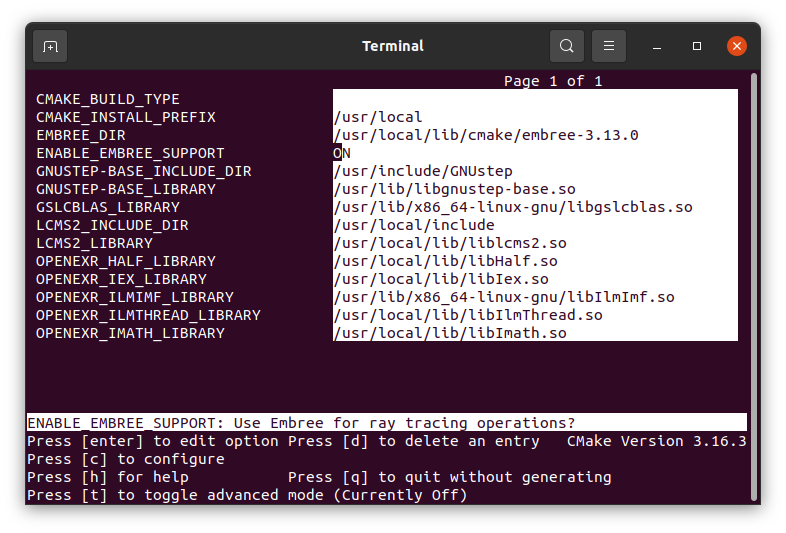
\includegraphics[width=.8\linewidth]{img/appendix/ccmake.png}
		\caption{Setting the \texttt{ENABLE\_EMBREE\_SUPPORT} in CCmake.}
		\label{fig:ccmake}
	\end{figure}
	 One can navigate through the table with the arrow keys. Locate the variable \texttt{ENABLE\_EMBREE\_SUPPORT} and press \texttt{ENTER} in order to set this variable from \texttt{OFF} to \texttt{ON}. Press \texttt{c} once again to re-configure the project and exit the "feedback screen" with \texttt{e}. Now, in the list of options at the bottom, an option \texttt{Press [g] to generate and exit} should be visible. Press \texttt{g} to generate the project and exit CCMake. 
	 
	 
	\item Continue following the steps in Chapter 2. 
	
	\item The functionality and usage of ART is the central topic of Chapter 3.
     \texttt{Arm} scene files are rendered by invoking the \emph{artist} command line tool. For an overview of the features and command line options, type
     \begin{Verbatim}
artist -h
     \end{Verbatim} 
     
	 A scene file, say \texttt{foo.arm}, with native ART can be rendered by typing
	 \begin{Verbatim}
artist foo.arm 
	 \end{Verbatim}
	 If Embree support is desired, artist has to be executed with an additional \texttt{-e} flag:
	 \begin{Verbatim}
artist foo.arm -e
	 \end{Verbatim}

	
\end{enumerate} 



\section{Installation of ART on Windows 10}
As briefly mentioned earlier, ART naturally does not support Windows platforms. However, with the help of a so-called Linux Subsystem for Windows, running ART on Windows 10 is possible. This section guides through the process of setting up such a subsystem and additional tools for displaying rendered images. In this section, the subsystem of choice is "Ubuntu 20.04 LTS".

\begin{enumerate}
	
	\item Begin by opening the Microsoft Store and type "Ubuntu" in the search bar on the top right. This should result in a display of multiple apps. Select the "Ubuntu 20.04 LTS" app like shown in Figure \ref{fig:ubuntu} and install it. 
	\begin{figure}[h]
		\centering
		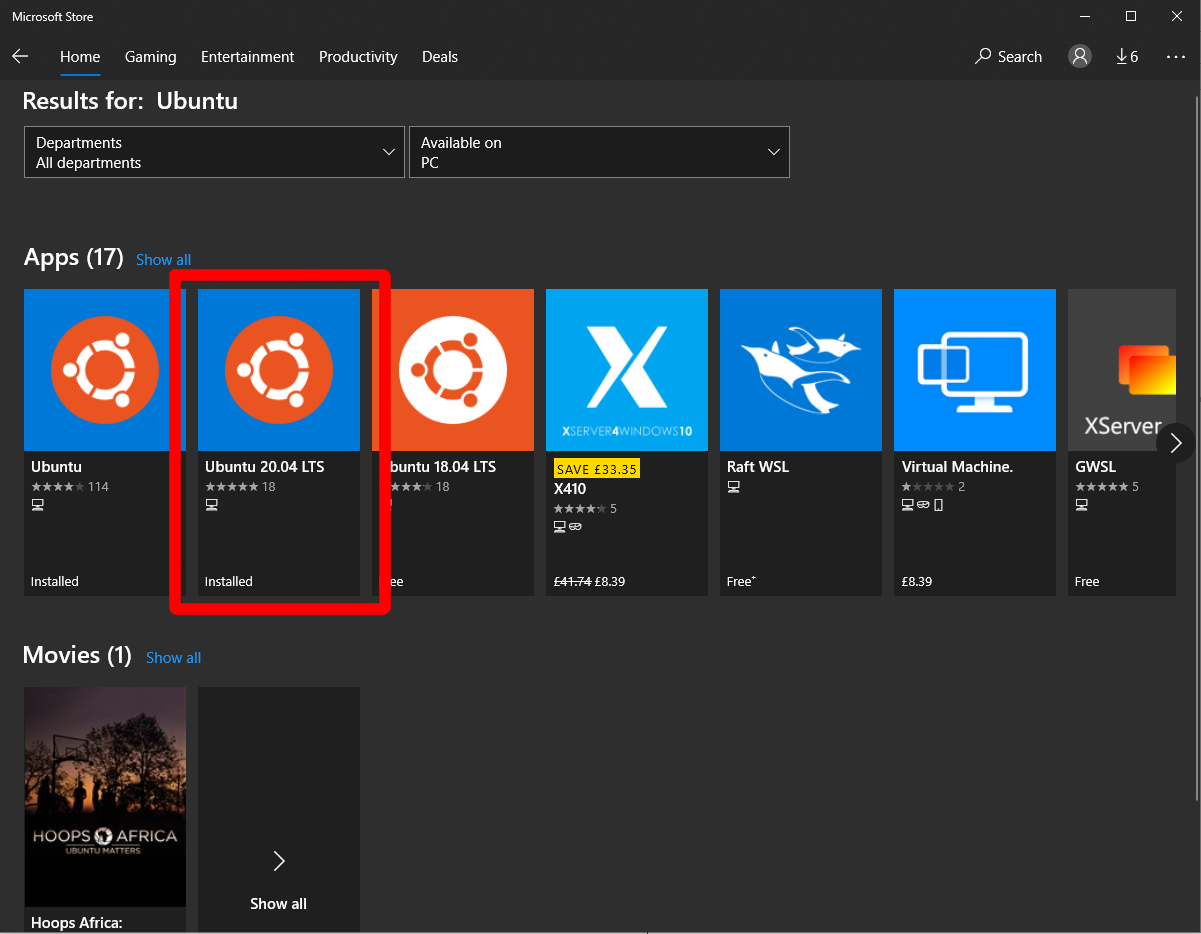
\includegraphics[width=.8\linewidth]{img/appendix/ubuntu.png}
		\caption{The Ubuntu subsystem we are using in the Microsoft Store.}
		\label{fig:ubuntu}
	\end{figure}
	
	\item After the installation, click the \texttt{Launch} button in the Microsoft Store. A terminal will open. Wait a few minutes until the setup is complete, and provide a user name and password.
	After that, the subsystem is up and ready.
	
	\item While being in the \emph{home/<username>} directory, type
	\begin{Verbatim}
		explorer.exe .
	\end{Verbatim}
	to open the Windows file explorer. Extract the zipped folder containing the ART source code here, or create a suitable location for it in the directory and extract it there.
	
	\item The Linux subsystem does not natively support graphics user interface applications, although these are crucial for viewing rendered images. However, displaying GUI-applications in general can be done by running an X server on Windows 10, which communicates to the Linux subsystem. The following procedure is taken from the guide \citetitle{windowsSubsystem} \cite{windowsSubsystem}. There is a variety of such X servers. Like the author of the guide, we decided to use \emph{Xming}. It can be downloaded via
	\emph{\href{https://sourceforge.net/projects/xming/}{https://sourceforge.net/projects/xming/}}.
	Download the executable and follow the installation wizzard, leave the settings as default. Start the application. An \texttt{XLaunch} should be visible in the Windows toolbar.
	\begin{figure}[h]
		\centering
		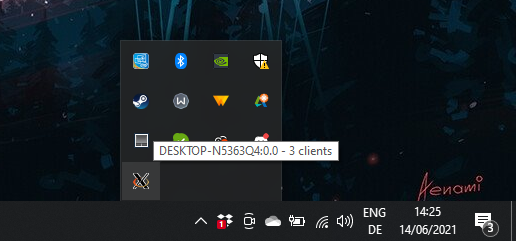
\includegraphics[width=.5\linewidth]{img/appendix/xlaunch.png}
		\caption{XLaunch running in the background.}
		\label{fig:xlaunch}
	\end{figure}  
	
	In the Ubuntu terminal, type
	\begin{Verbatim}
export DISPLAY=:0
	\end{Verbatim}
	This will enable the display of graphical user interfaces from the Linux subsystem in Windows.
	
	
	\item Follow the instructions in Section \ref{embree} and \ref{art} to setup Embree and ART.
	
\begin{figure}[h]
	\centering
	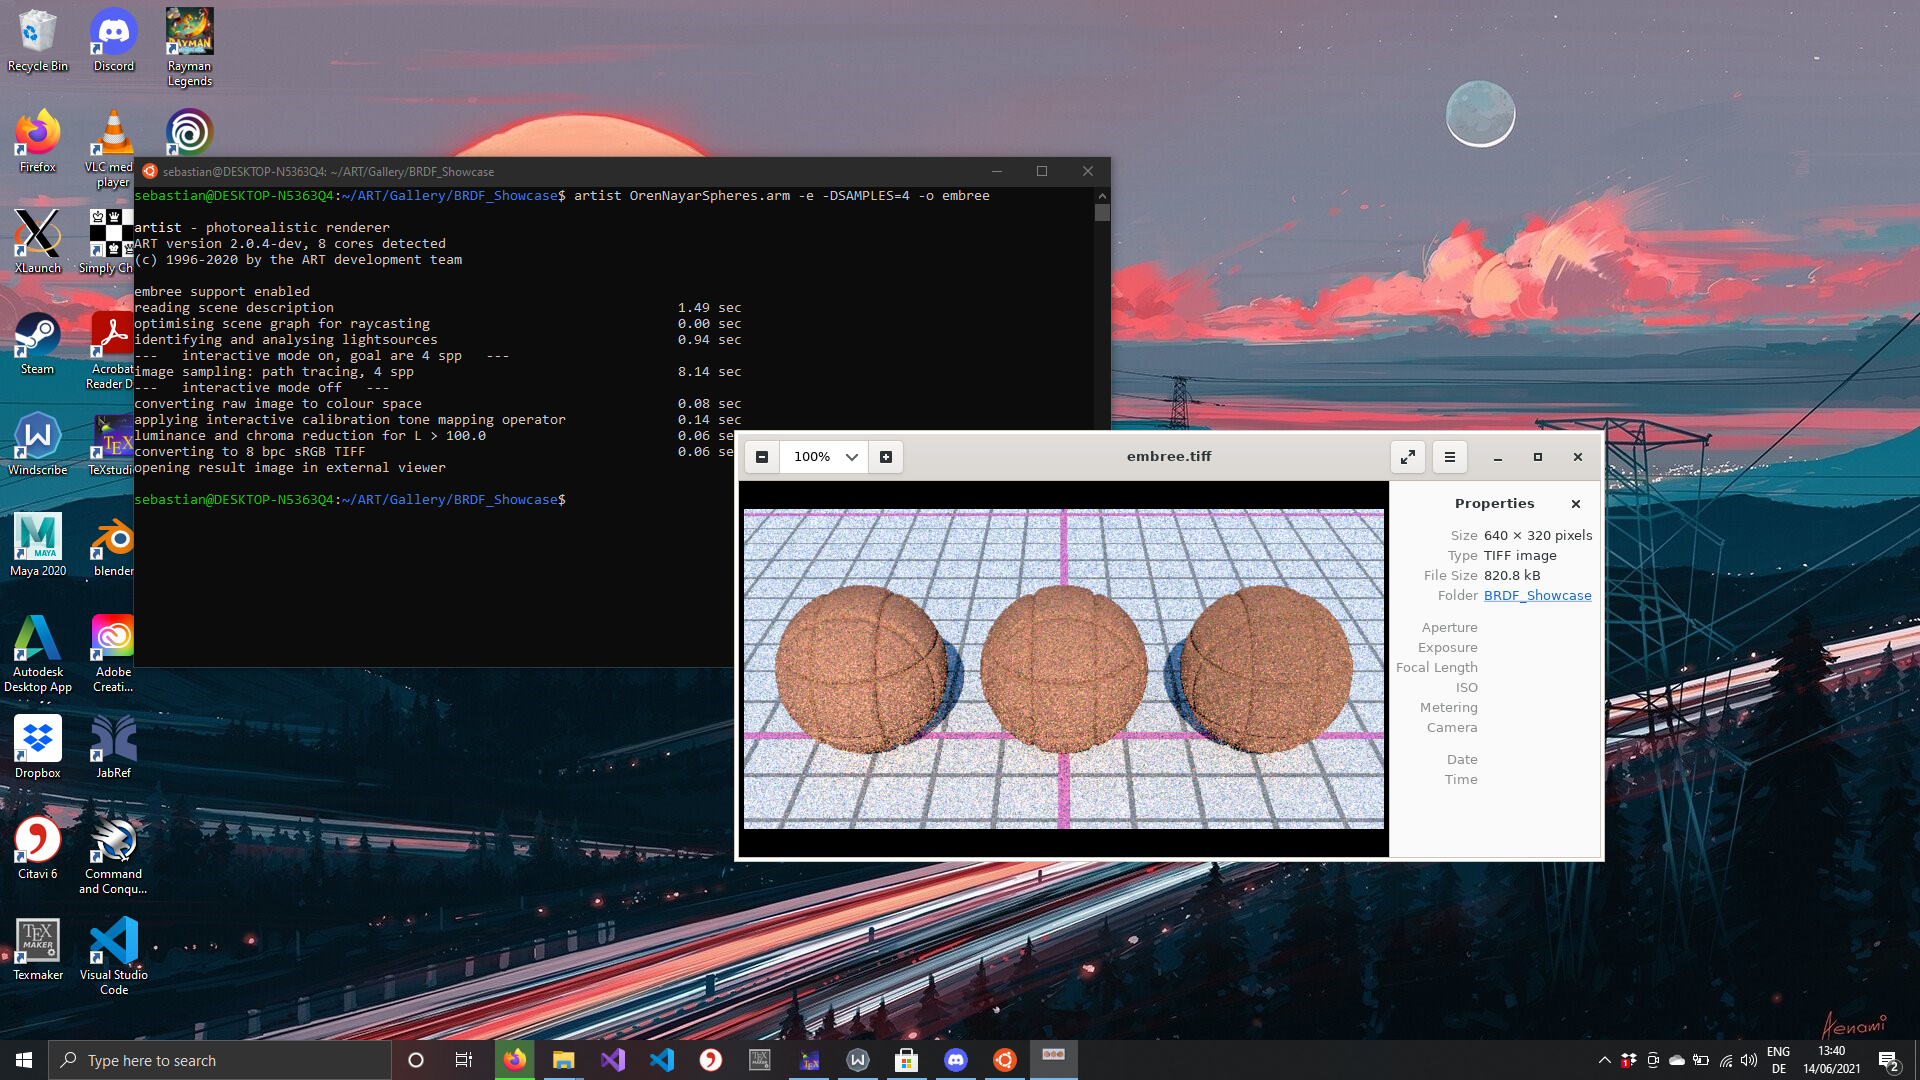
\includegraphics[width=1\linewidth]{img/appendix/final.png}
	\caption{Rendering with ART on Windows 10.}
	\label{fig:final}
\end{figure}
	
	
\end{enumerate}
